\section[Desenvolvimento do Projeto]{Desenvolvimento do Projeto}

\subsection{Repositório do Código Fonte do Projeto}
Para este projeto foram utilizados dois repositórios para código e um para a wiki, todos foram mantidos no GitLab da AGES. A separação dos repositórios de código foi feita em frontend, o qual utiliza a tecnologia Flutter\cite{flutter}, usando a linguagem Dart\cite{dart} e backend, que utiliza as tecnologias NodeJs\cite{nodejs} e ExpressJs\cite{expressjs}, usando a linguagem JavaScript\cite{javascript} e TypeScript\cite{typescript}

\begin{itemize}
  \item Sow Good wiki: https://tools.ages.pucrs.br/sow-good/wiki/-/wikis/home
  \item Sow Good frontend: https://tools.ages.pucrs.br/sow-good/sow-good-frontend
  \item Sow Good backend: https://tools.ages.pucrs.br/sow-good/sow-good-backend
\end{itemize}

\subsection{Banco de Dados Utilizado}
Inicialmente foi pensado em utilizar um banco de dados relacional para a realização do projeto por conta da sua simplicidade e ser conhecido por todos integrantes da equipe, porém, com o andamento da Sprint 0 foi decidido que seria melhor utilizar um dos bancos de dados disponibilizados pelo Firebase, dado que estaríamos utilizando o Firebase Authentication, um produto que iria fazer a criação e autenticação dos usuários, além de guardar informações críticas de forma segura, o que iria nos facilitar na parte de cadastro e login dos usuários.

Dentre as opções diponibilizadas pelo Firebase, acabamos escolhendo o Firestore\cite{firestore} Database que é o banco de dados não relacional disponibilizado pela Firebase\cite{firebase}. Uma outra opção seria utilizar o Realtime Database\cite{realtimedb}, que também utiliza o esquema não relacional, porém, alguns integrantes da equipe ja possuíam experiência com o Firestore\cite{firestore}, sendo esse, o motivo pelo qual escolhemos utilizá-lo.

\begin{figure}[H]
    \centering
    \small
    \caption{Esquema Conceitual Banco de Dados Sow Good}
    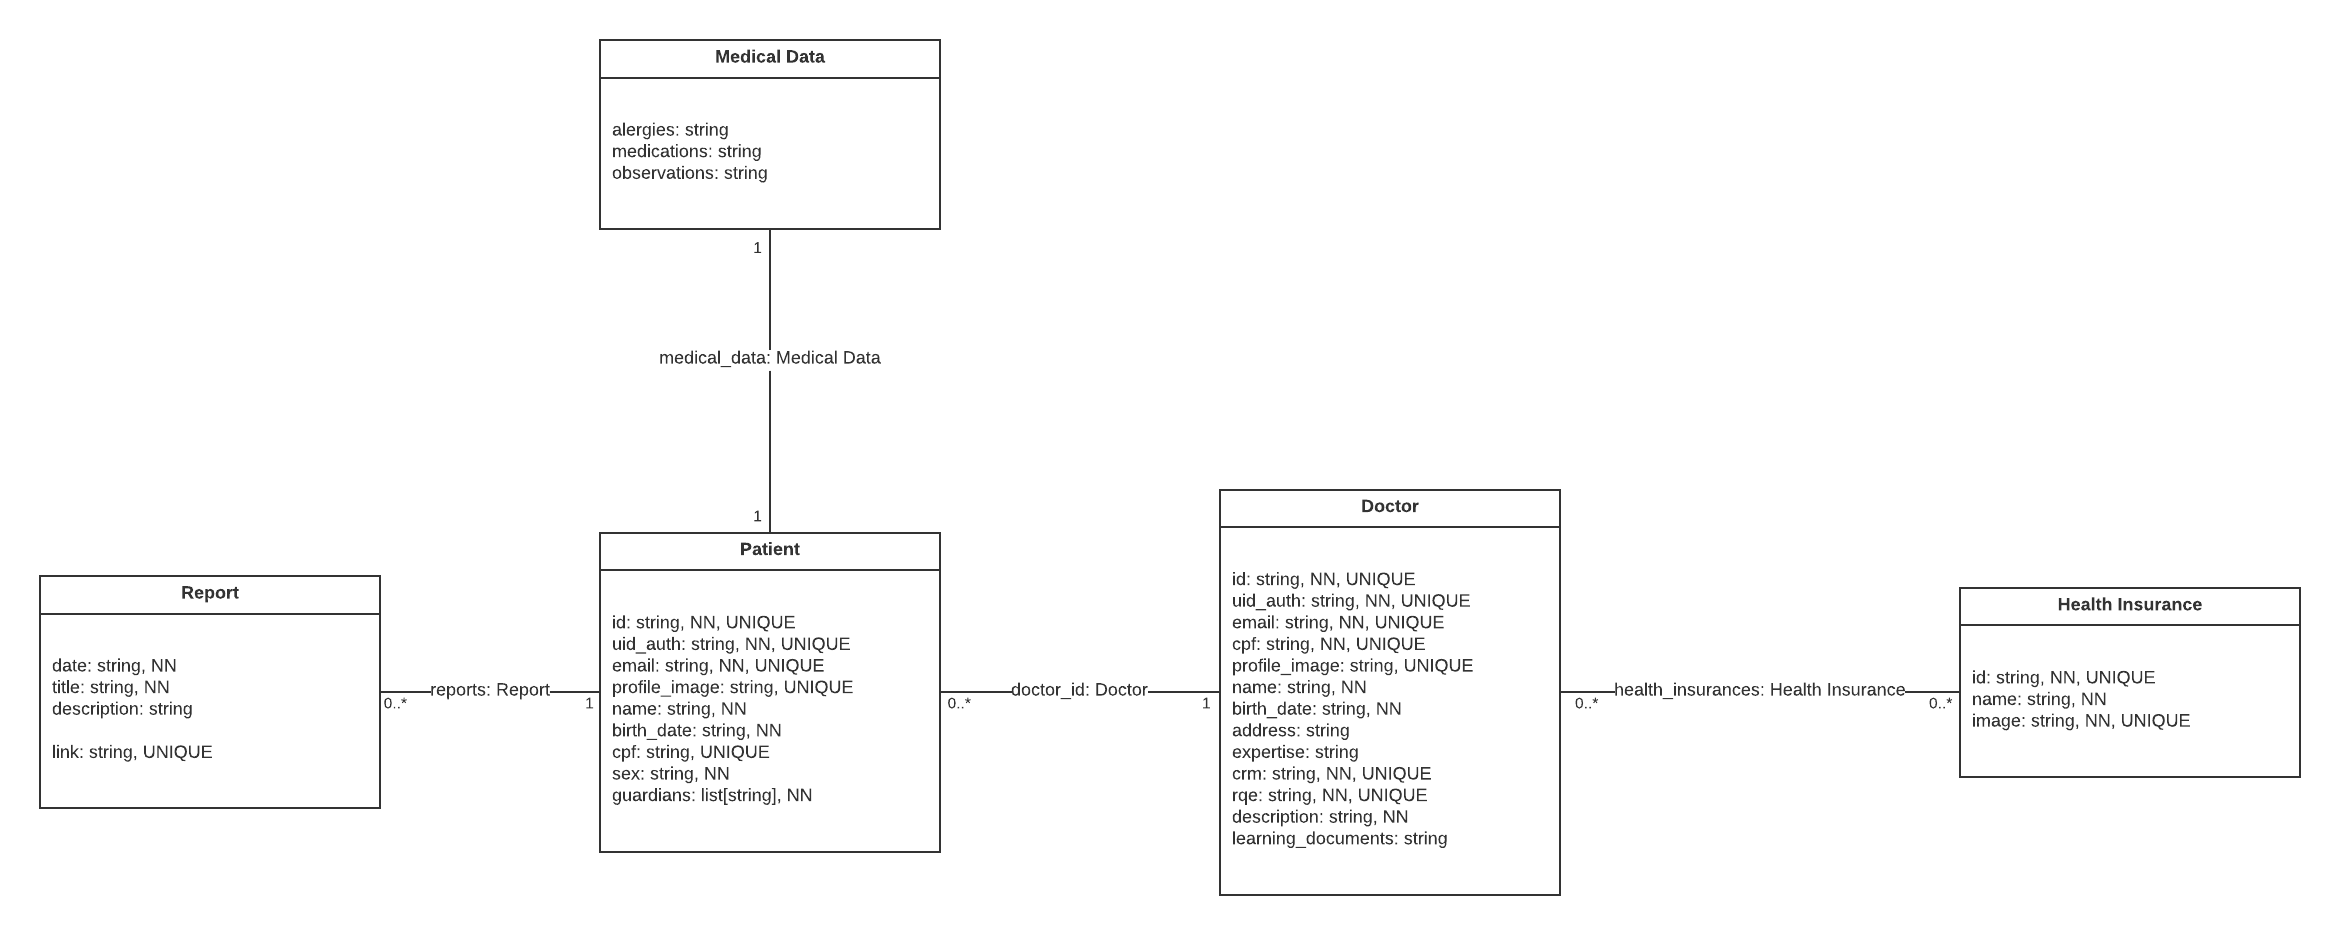
\includegraphics[width=1\linewidth]{conteudo//3 - ages II//conteudo//figures//bd-conceitual.png}
    Fonte: https://tools.ages.pucrs.br/sow-good/wiki/-/wikis/banco\_dados
\end{figure}

\subsection{Arquitetura Utilizada}
A arquitetura, assim como foi na AGES I, segue o modelo cliente-servidor 
que consiste em três partes principais, o banco de dados, onde são guardados todos 
dados necessários para o funcionamento correto do sistema, o servidor que conecta 
o cliente ao banco de dados, fazendo toda a transformação do tipo de dados e 
tratamento necessários, assim devolvendo uma informação utilizável pelo cliente que 
é a última parte do modelo e o cliente, que é responsável por apresentar as informações recebidas do servidor através de uma interface gráfica de fácil utilização.

\begin{figure}[H]
    \centering
    \small
    \caption{Arquitetura Geral Sow Good}
    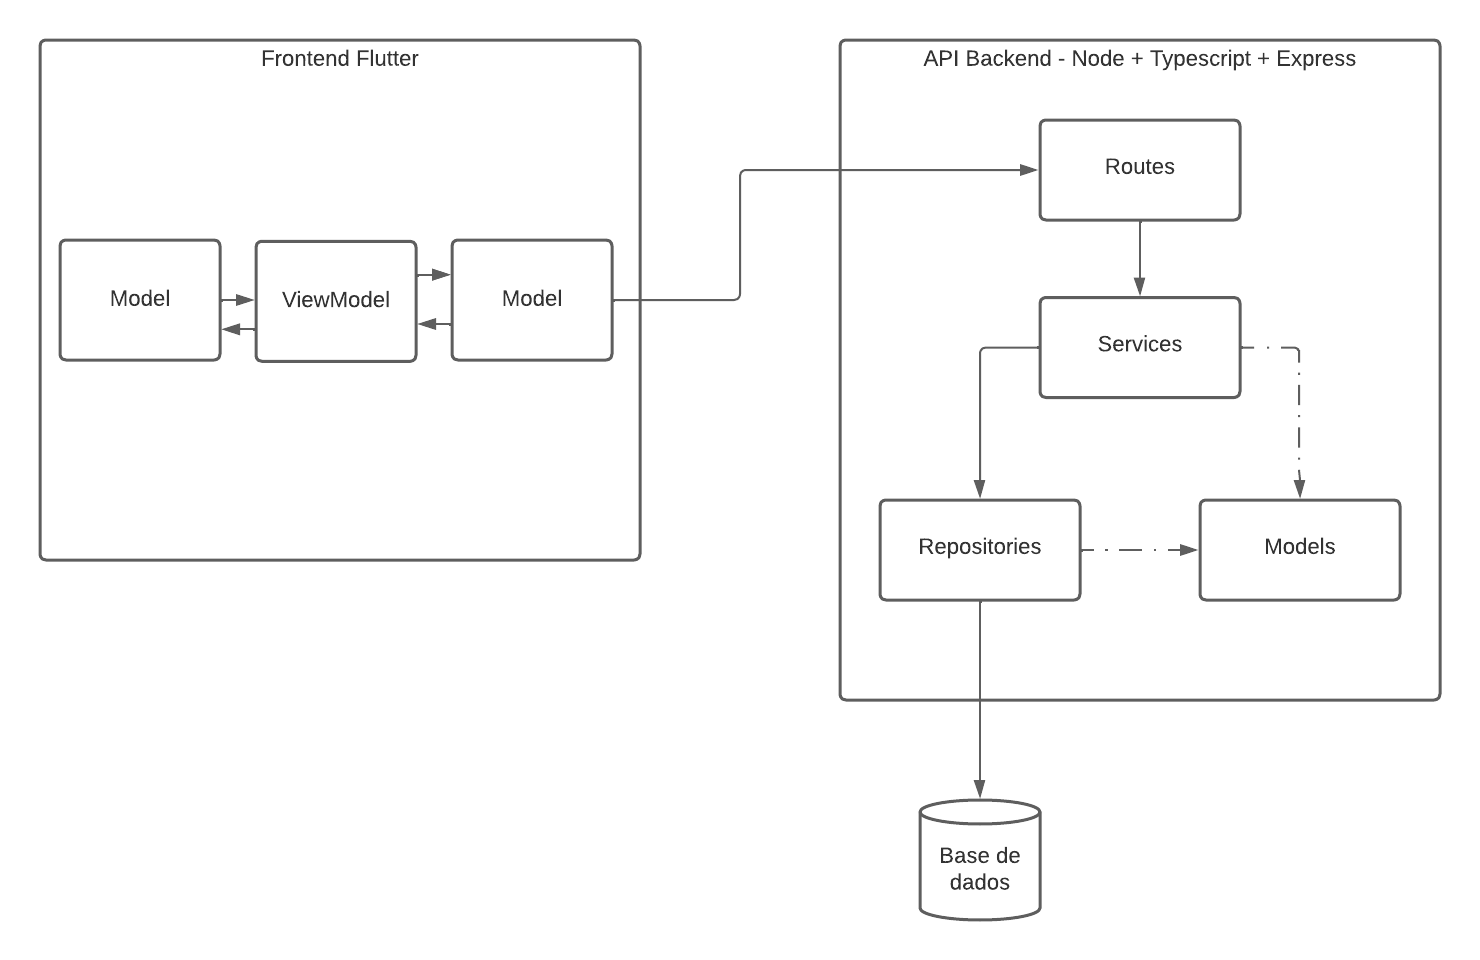
\includegraphics[width=1\linewidth]{conteudo//3 - ages II//conteudo//figures//arquitetura-geral.png}
    Fonte: https://tools.ages.pucrs.br/sow-good/wiki/-/wikis/arquitetura
\end{figure}

\subsection{Protótipos das Telas Desenvolvidas}
Dado que inicialmente o projeto ainda não possuía uma identidade visual bem 
definida, seguimos padrões de design mais comumente utilizados, como, por exemplo, componentes mais arredondados, um bom contraste de cores para que o aplicativo pudesse ser utilizado 
por pessoas com problemas visuais com facilidade e tamanho e cor de letras para 
permitir uma leitura fácil. Para produzir os protótipos foi usada a plataforma Figma\cite{figma}, que permite que várias pessoas desenvolvam simultaneamente, diminuindo a quantidade de retrabalho e aumentando a eficiênciado time.

\begin{itemize}
  \item https://tools.ages.pucrs.br/sow-good/wiki/-/wikis/mockups
\end{itemize}

\subsection{Tecnologias Utilizadas}

O projeto foi construído utilizando cinco tecnologias diferentes, sendo elas o 
Flutter\cite{flutter} com a linguagem Dart\cite{dart} para o frontend, o NodeJs\cite{nodejs} para o backend utilizando ExpressJs\cite{expressjs} para lidar com os diferentes endpoints existentes na \ac{api}, o Firebase Authentication\cite{firebaseauth} para lidar com cadastro e login de usuários e Firestore\cite{firestore} como banco de dados.

A escolha do Flutter\cite{flutter} para o frontend foi feita pois é uma das tecnologias que 
permite o desenvolvimento de aplicações para Android, IOS e Web em uma única 
linguagem, diminuindo, assim, o estudo e trabalho necessário para o desenvolvimento 
do projeto.

Para o backend foi escolhido o NodeJs\cite{nodejs} por ser uma tecnologia muito utilizada 
atualmente e por diversos integrantes da equipe possuir um conhecimento prévio 
acerca da ferramenta, assim, podendo ajudar quem estiver tendo problemas. O uso 
do ExpressJs\cite{expressjs} foi feito para que pudesse haver uma maneira mais organizada de definir cada endpoint existente na nossa \ac{api}. 

O Firebase Authentication\cite{firebaseauth} foi utilizado para facilitar e diminuir o trabalho 
necessário para a implementação de um sistema de autenticação, permitindo que a equipe foque em outros pontos importantes da aplicação. 

O Firestore\cite{firestore}, assim como o NodeJs\cite{nodejs}, foi escolhido por alguns 
integrantes da equipe já possuir conhecimento prévio acerca da ferramenta, e, 
também, por ser, assim como o Firebase Authentication\cite{firebaseauth} e o Flutter\cite{flutter}, uma tecnologia desenvolvida pela Google\cite{google}, ou seja, elas possuem grande compatibilidade entre sí.